\documentclass[]{article}
\usepackage{lmodern}
\usepackage{amssymb,amsmath}
\usepackage{ifxetex,ifluatex}
\usepackage{fixltx2e} % provides \textsubscript
\ifnum 0\ifxetex 1\fi\ifluatex 1\fi=0 % if pdftex
  \usepackage[T1]{fontenc}
  \usepackage[utf8]{inputenc}
\else % if luatex or xelatex
  \ifxetex
    \usepackage{mathspec}
  \else
    \usepackage{fontspec}
  \fi
  \defaultfontfeatures{Ligatures=TeX,Scale=MatchLowercase}
\fi
% use upquote if available, for straight quotes in verbatim environments
\IfFileExists{upquote.sty}{\usepackage{upquote}}{}
% use microtype if available
\IfFileExists{microtype.sty}{%
\usepackage{microtype}
\UseMicrotypeSet[protrusion]{basicmath} % disable protrusion for tt fonts
}{}
\usepackage[margin=1in]{geometry}
\usepackage{hyperref}
\hypersetup{unicode=true,
            pdftitle={My Running Data},
            pdfauthor={Dan Spencer},
            pdfborder={0 0 0},
            breaklinks=true}
\urlstyle{same}  % don't use monospace font for urls
\usepackage{color}
\usepackage{fancyvrb}
\newcommand{\VerbBar}{|}
\newcommand{\VERB}{\Verb[commandchars=\\\{\}]}
\DefineVerbatimEnvironment{Highlighting}{Verbatim}{commandchars=\\\{\}}
% Add ',fontsize=\small' for more characters per line
\usepackage{framed}
\definecolor{shadecolor}{RGB}{248,248,248}
\newenvironment{Shaded}{\begin{snugshade}}{\end{snugshade}}
\newcommand{\AlertTok}[1]{\textcolor[rgb]{0.94,0.16,0.16}{#1}}
\newcommand{\AnnotationTok}[1]{\textcolor[rgb]{0.56,0.35,0.01}{\textbf{\textit{#1}}}}
\newcommand{\AttributeTok}[1]{\textcolor[rgb]{0.77,0.63,0.00}{#1}}
\newcommand{\BaseNTok}[1]{\textcolor[rgb]{0.00,0.00,0.81}{#1}}
\newcommand{\BuiltInTok}[1]{#1}
\newcommand{\CharTok}[1]{\textcolor[rgb]{0.31,0.60,0.02}{#1}}
\newcommand{\CommentTok}[1]{\textcolor[rgb]{0.56,0.35,0.01}{\textit{#1}}}
\newcommand{\CommentVarTok}[1]{\textcolor[rgb]{0.56,0.35,0.01}{\textbf{\textit{#1}}}}
\newcommand{\ConstantTok}[1]{\textcolor[rgb]{0.00,0.00,0.00}{#1}}
\newcommand{\ControlFlowTok}[1]{\textcolor[rgb]{0.13,0.29,0.53}{\textbf{#1}}}
\newcommand{\DataTypeTok}[1]{\textcolor[rgb]{0.13,0.29,0.53}{#1}}
\newcommand{\DecValTok}[1]{\textcolor[rgb]{0.00,0.00,0.81}{#1}}
\newcommand{\DocumentationTok}[1]{\textcolor[rgb]{0.56,0.35,0.01}{\textbf{\textit{#1}}}}
\newcommand{\ErrorTok}[1]{\textcolor[rgb]{0.64,0.00,0.00}{\textbf{#1}}}
\newcommand{\ExtensionTok}[1]{#1}
\newcommand{\FloatTok}[1]{\textcolor[rgb]{0.00,0.00,0.81}{#1}}
\newcommand{\FunctionTok}[1]{\textcolor[rgb]{0.00,0.00,0.00}{#1}}
\newcommand{\ImportTok}[1]{#1}
\newcommand{\InformationTok}[1]{\textcolor[rgb]{0.56,0.35,0.01}{\textbf{\textit{#1}}}}
\newcommand{\KeywordTok}[1]{\textcolor[rgb]{0.13,0.29,0.53}{\textbf{#1}}}
\newcommand{\NormalTok}[1]{#1}
\newcommand{\OperatorTok}[1]{\textcolor[rgb]{0.81,0.36,0.00}{\textbf{#1}}}
\newcommand{\OtherTok}[1]{\textcolor[rgb]{0.56,0.35,0.01}{#1}}
\newcommand{\PreprocessorTok}[1]{\textcolor[rgb]{0.56,0.35,0.01}{\textit{#1}}}
\newcommand{\RegionMarkerTok}[1]{#1}
\newcommand{\SpecialCharTok}[1]{\textcolor[rgb]{0.00,0.00,0.00}{#1}}
\newcommand{\SpecialStringTok}[1]{\textcolor[rgb]{0.31,0.60,0.02}{#1}}
\newcommand{\StringTok}[1]{\textcolor[rgb]{0.31,0.60,0.02}{#1}}
\newcommand{\VariableTok}[1]{\textcolor[rgb]{0.00,0.00,0.00}{#1}}
\newcommand{\VerbatimStringTok}[1]{\textcolor[rgb]{0.31,0.60,0.02}{#1}}
\newcommand{\WarningTok}[1]{\textcolor[rgb]{0.56,0.35,0.01}{\textbf{\textit{#1}}}}
\usepackage{graphicx,grffile}
\makeatletter
\def\maxwidth{\ifdim\Gin@nat@width>\linewidth\linewidth\else\Gin@nat@width\fi}
\def\maxheight{\ifdim\Gin@nat@height>\textheight\textheight\else\Gin@nat@height\fi}
\makeatother
% Scale images if necessary, so that they will not overflow the page
% margins by default, and it is still possible to overwrite the defaults
% using explicit options in \includegraphics[width, height, ...]{}
\setkeys{Gin}{width=\maxwidth,height=\maxheight,keepaspectratio}
\IfFileExists{parskip.sty}{%
\usepackage{parskip}
}{% else
\setlength{\parindent}{0pt}
\setlength{\parskip}{6pt plus 2pt minus 1pt}
}
\setlength{\emergencystretch}{3em}  % prevent overfull lines
\providecommand{\tightlist}{%
  \setlength{\itemsep}{0pt}\setlength{\parskip}{0pt}}
\setcounter{secnumdepth}{0}
% Redefines (sub)paragraphs to behave more like sections
\ifx\paragraph\undefined\else
\let\oldparagraph\paragraph
\renewcommand{\paragraph}[1]{\oldparagraph{#1}\mbox{}}
\fi
\ifx\subparagraph\undefined\else
\let\oldsubparagraph\subparagraph
\renewcommand{\subparagraph}[1]{\oldsubparagraph{#1}\mbox{}}
\fi

%%% Use protect on footnotes to avoid problems with footnotes in titles
\let\rmarkdownfootnote\footnote%
\def\footnote{\protect\rmarkdownfootnote}

%%% Change title format to be more compact
\usepackage{titling}

% Create subtitle command for use in maketitle
\providecommand{\subtitle}[1]{
  \posttitle{
    \begin{center}\large#1\end{center}
    }
}

\setlength{\droptitle}{-2em}

  \title{My Running Data}
    \pretitle{\vspace{\droptitle}\centering\huge}
  \posttitle{\par}
    \author{Dan Spencer}
    \preauthor{\centering\large\emph}
  \postauthor{\par}
    \date{}
    \predate{}\postdate{}
  

\begin{document}
\maketitle

\hypertarget{background}{%
\subsection{Background}\label{background}}

I got into running a few years ago after spending too many long days
working at a desk. In December 2016, I began tracking my runs using a
running app called Strava. I started using this particular run-tracking
app because I found that it does a pretty good job keeping track of all
sorts of data, which you can then access yourself at a later date. In
this particular document, I'll be cleaning my data aggregated by
workout, creating a visualization to see if my speed is changing
significantly over time, and then comparing my different runs to
determine whether different shoes have a significant effect on my pace.

\hypertarget{cleaning-the-data}{%
\subsection{Cleaning the Data}\label{cleaning-the-data}}

I downloaded my data directly from
\href{https://www.strava.com/}{Strava}, and it came in a folder called
\texttt{export\_18831425}. Within this folder area number of
spreadsheets and subfolders. I will focus on the \texttt{activities.csv}
spreasheet for my analysis here.

\begin{Shaded}
\begin{Highlighting}[]
\NormalTok{activities <-}\StringTok{ }\KeywordTok{read.csv}\NormalTok{(}\StringTok{"export_18831425/activities.csv"}\NormalTok{)}
\KeywordTok{names}\NormalTok{(activities) }\CommentTok{# This gives the names of the variables in the spreadsheet}
\end{Highlighting}
\end{Shaded}

\begin{verbatim}
##  [1] "Activity.ID"          "Activity.Date"        "Activity.Name"       
##  [4] "Activity.Type"        "Activity.Description" "Elapsed.Time"        
##  [7] "Distance"             "Relative.Effort"      "Commute"             
## [10] "Activity.Gear"        "Filename"
\end{verbatim}

\begin{Shaded}
\begin{Highlighting}[]
\KeywordTok{table}\NormalTok{(activities}\OperatorTok{$}\NormalTok{Activity.Type)}
\end{Highlighting}
\end{Shaded}

\begin{verbatim}
## 
##  E-Bike Ride         Ride          Run Virtual Ride 
##            3            6          366            1
\end{verbatim}

My efforts today will focus on my running activities, and I'll only need
to look at the \texttt{Activity.Date}, \texttt{Activity.Gear},
\texttt{Elapsed.Time}, and \texttt{Distance} variables, so I will begin
by cleaning the data to match my needs.

\begin{Shaded}
\begin{Highlighting}[]
\KeywordTok{library}\NormalTok{(tidyverse)}
\NormalTok{run_df <-}\StringTok{ }\NormalTok{activities }\OperatorTok\StringTok{ }
\StringTok{  }\NormalTok{dplyr}\OperatorTok{::}\KeywordTok{filter}\NormalTok{(Activity.Type }\OperatorTok{==}\StringTok{ "Run"}\NormalTok{) }\OperatorTok\StringTok{ }\CommentTok{# Only look at runs}
\StringTok{  }\NormalTok{dplyr}\OperatorTok{::}\KeywordTok{select}\NormalTok{(Activity.Date, Activity.Gear, Elapsed.Time, Distance)}
\KeywordTok{head}\NormalTok{(run_df)}
\end{Highlighting}
\end{Shaded}

\begin{verbatim}
##               Activity.Date Activity.Gear Elapsed.Time Distance
## 1  Dec 14, 2016, 5:22:14 PM                       2208     8.05
## 2  Dec 16, 2016, 4:48:25 PM                       2230     7.95
## 3 Dec 17, 2016, 10:20:49 PM                       2102     7.94
## 4  Dec 18, 2016, 5:43:09 PM                       2169     8.04
## 5  Dec 21, 2016, 2:41:48 PM                       2750     9.43
## 6  Dec 22, 2016, 4:36:18 PM                       3063    10.44
\end{verbatim}

Something that I notice here is that the \texttt{Activity.Date} variable
is not in a standard format. Since I'm only interested in the date when
the runs took place, I can try to format the dates into a date format
that can be recognized by R. I can also convert the
\texttt{Elapsed.Time} from seconds to minutes, convert \texttt{Distance}
from kilometers to miles, and find my pace by dividing the time in
minutes by the distance in miles. I'll sum up the distances and times
for any activities that occur on the same day to ensure I have a unique
daily value.

\begin{Shaded}
\begin{Highlighting}[]
\NormalTok{final_run_df <-}\StringTok{ }\NormalTok{run_df }\OperatorTok\StringTok{ }
\StringTok{  }\NormalTok{dplyr}\OperatorTok{::}\KeywordTok{mutate}\NormalTok{(}\DataTypeTok{Date =} \KeywordTok{substr}\NormalTok{(Activity.Date,}\DecValTok{1}\NormalTok{,}\DecValTok{12}\NormalTok{), }\CommentTok{# Get rid of the time information}
                \DataTypeTok{Date =} \KeywordTok{as.Date}\NormalTok{(Date,}\DataTypeTok{format =} \StringTok{"%b %d, %Y"}\NormalTok{)) }\OperatorTok\StringTok{  }\CommentTok{# Get R to read as a date}
\StringTok{  }\NormalTok{dplyr}\OperatorTok{::}\KeywordTok{group_by}\NormalTok{(Date) }\OperatorTok\StringTok{ }\CommentTok{# Next, in case there are multiple runs in a day, group all of the data together}
\StringTok{  }\NormalTok{dplyr}\OperatorTok{::}\KeywordTok{summarize}\NormalTok{(}\DataTypeTok{Elapsed.Time =} \KeywordTok{sum}\NormalTok{(Elapsed.Time),}
                   \DataTypeTok{Distance =} \KeywordTok{sum}\NormalTok{(Distance),}
                   \DataTypeTok{Activity.Gear =} \KeywordTok{first}\NormalTok{(Activity.Gear)) }\OperatorTok\StringTok{ }
\StringTok{  }\NormalTok{dplyr}\OperatorTok{::}\KeywordTok{ungroup}\NormalTok{() }\OperatorTok\StringTok{ }
\StringTok{  }\NormalTok{dplyr}\OperatorTok{::}\KeywordTok{mutate}\NormalTok{(}\DataTypeTok{Distance =}\NormalTok{ Distance }\OperatorTok{/}\StringTok{ }\FloatTok{1.609}\NormalTok{, }\CommentTok{# Convert from km to miles}
                \DataTypeTok{Minutes =}\NormalTok{ Elapsed.Time }\OperatorTok{/}\StringTok{ }\DecValTok{60}\NormalTok{, }\CommentTok{# Convert from second to minutes}
                \DataTypeTok{Pace =}\NormalTok{ Minutes }\OperatorTok{/}\StringTok{ }\NormalTok{Distance)}
\end{Highlighting}
\end{Shaded}

\hypertarget{visualizing-my-pace-through-time}{%
\subsection{Visualizing My Pace Through
Time}\label{visualizing-my-pace-through-time}}

It might be interesting to see if I have gotten faster or slower through
time over the past few years. Am I getting slower as I get older?

\begin{Shaded}
\begin{Highlighting}[]
\KeywordTok{ggplot}\NormalTok{(final_run_df) }\OperatorTok{+}
\StringTok{  }\KeywordTok{geom_point}\NormalTok{(}\KeywordTok{aes}\NormalTok{(}\DataTypeTok{x =}\NormalTok{ Date, }\DataTypeTok{y =}\NormalTok{ Pace)) }\OperatorTok{+}\StringTok{ }\CommentTok{# Put the points on the graph}
\StringTok{  }\KeywordTok{geom_smooth}\NormalTok{(}\KeywordTok{aes}\NormalTok{(}\DataTypeTok{x =}\NormalTok{ Date, }\DataTypeTok{y =}\NormalTok{ Pace)) }\OperatorTok{+}\StringTok{ }\CommentTok{# Plot a smoothed curve over the points}
\StringTok{  }\KeywordTok{scale_y_continuous}\NormalTok{(}\StringTok{"Pace}\CharTok{\textbackslash{}n}\StringTok{(minutes per mile)"}\NormalTok{,}\DataTypeTok{breaks =} \KeywordTok{seq}\NormalTok{(}\DecValTok{6}\NormalTok{,}\DecValTok{17}\NormalTok{)) }\OperatorTok{+}\StringTok{ }\CommentTok{# Control where the grid lines are on the y-axis}
\StringTok{  }\KeywordTok{ggtitle}\NormalTok{(}\StringTok{"Am I getting slower?"}\NormalTok{) }\OperatorTok{+}\StringTok{ }\CommentTok{# Adds a title}
\StringTok{  }\KeywordTok{theme_bw}\NormalTok{() }\CommentTok{# Gives a nice, clean plot with minimal color}
\end{Highlighting}
\end{Shaded}

\begin{verbatim}
## `geom_smooth()` using method = 'loess' and formula 'y ~ x'
\end{verbatim}

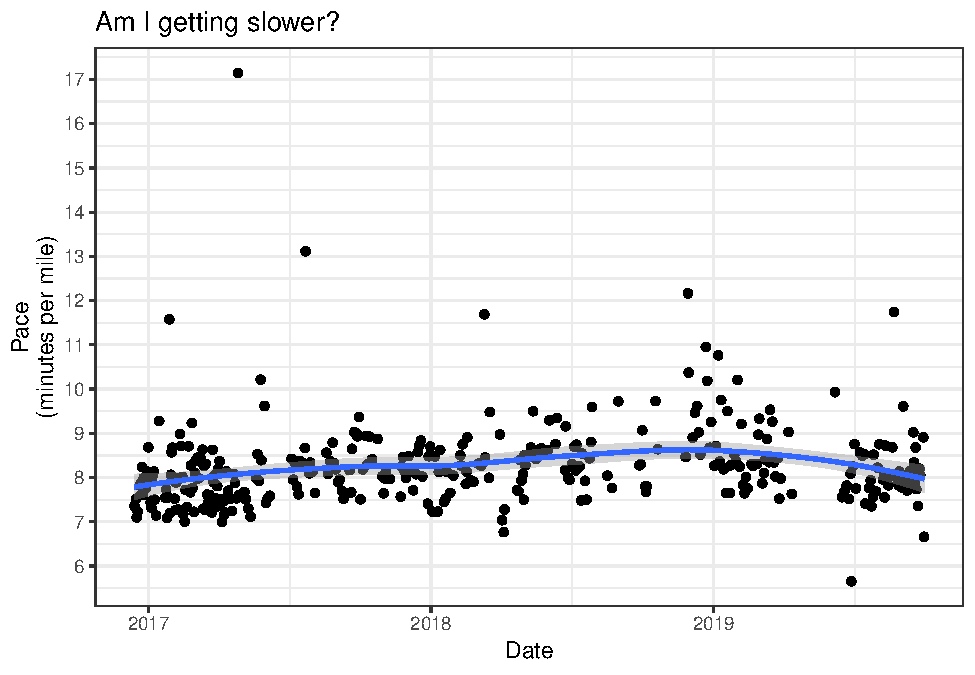
\includegraphics{my_running_data_files/figure-latex/unnamed-chunk-4-1.pdf}

These data suggest that I was getting slower through time until around
the beginning of 2019, when the trend reversed slightly. There are some
hidden pieces of information here. First, I suffered an injury to my
ankle in the summer of 2018, which slowed me down significantly as I
recovered. I also suffered a mild muscle strain around March of 2019,
which stopped my running completely for about two months. However, after
my recovery I have taken smaller runs at a faster pace.

\hypertarget{visualizing-distances-per-day-through-time}{%
\subsection{Visualizing Distances per Day Through
Time}\label{visualizing-distances-per-day-through-time}}

Something that has a large effect on pace is distance traveled. To this
end, I can examine how the distances I have run have changed over time.

\begin{Shaded}
\begin{Highlighting}[]
\KeywordTok{ggplot}\NormalTok{(final_run_df) }\OperatorTok{+}
\StringTok{  }\KeywordTok{geom_point}\NormalTok{(}\KeywordTok{aes}\NormalTok{(}\DataTypeTok{x =}\NormalTok{ Date, }\DataTypeTok{y =}\NormalTok{ Distance)) }\OperatorTok{+}\StringTok{ }\CommentTok{# Put the points on the graph}
\StringTok{  }\KeywordTok{geom_smooth}\NormalTok{(}\KeywordTok{aes}\NormalTok{(}\DataTypeTok{x =}\NormalTok{ Date, }\DataTypeTok{y =}\NormalTok{ Distance)) }\OperatorTok{+}\StringTok{ }\CommentTok{# Plot a smoothed curve over the points}
\StringTok{  }\KeywordTok{scale_y_continuous}\NormalTok{(}\StringTok{"Distance}\CharTok{\textbackslash{}n}\StringTok{(miles)"}\NormalTok{) }\OperatorTok{+}\StringTok{ }\CommentTok{# Control where the grid lines are on the y-axis}
\StringTok{  }\KeywordTok{ggtitle}\NormalTok{(}\StringTok{"Am I running less distance?"}\NormalTok{) }\OperatorTok{+}\StringTok{ }\CommentTok{# Adds a title}
\StringTok{  }\KeywordTok{theme_bw}\NormalTok{() }\CommentTok{# Gives a nice, clean plot with minimal color}
\end{Highlighting}
\end{Shaded}

\begin{verbatim}
## `geom_smooth()` using method = 'loess' and formula 'y ~ x'
\end{verbatim}

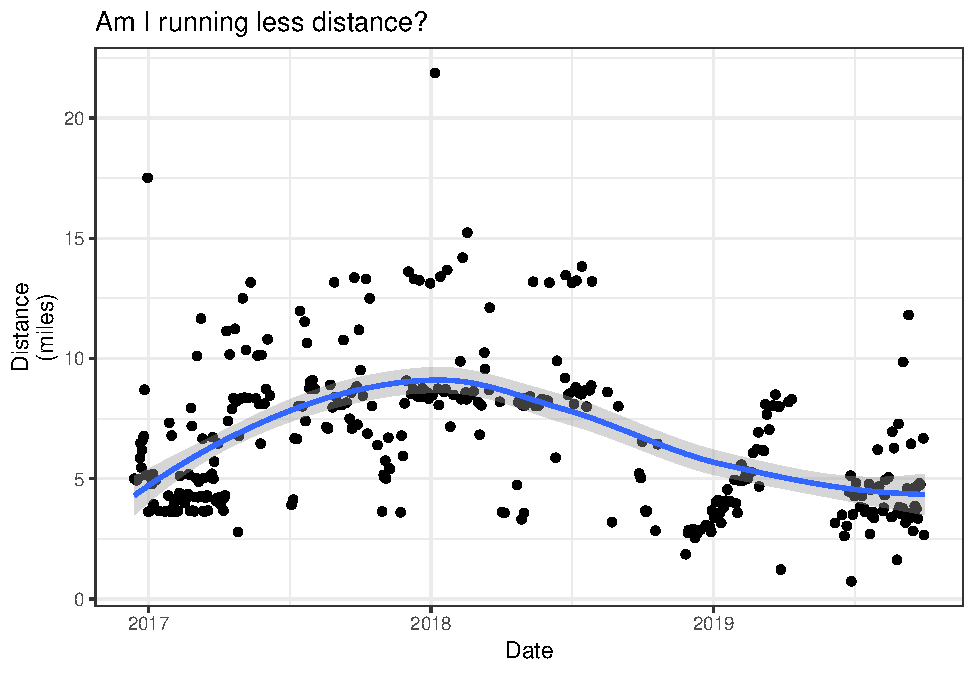
\includegraphics{my_running_data_files/figure-latex/unnamed-chunk-5-1.pdf}

From this plot, it's clear that I am running less on average in a given
day. My injuries and recoveries are also clearly observable, as my
distance drops down after each injury.

\hypertarget{do-the-shoes-make-a-difference}{%
\subsection{Do the Shoes Make a
Difference?}\label{do-the-shoes-make-a-difference}}

Now I'll see if I given pair of shoes makes me faster or slower. I'll
begin by looking at a visualization of the data to see if there could be
a difference.

\begin{Shaded}
\begin{Highlighting}[]
\NormalTok{shoes_df <-}\StringTok{ }\NormalTok{final_run_df }\OperatorTok\StringTok{ }
\StringTok{  }\NormalTok{dplyr}\OperatorTok{::}\KeywordTok{filter}\NormalTok{(Activity.Gear }\OperatorTok{!=}\StringTok{ ""}\NormalTok{) }\OperatorTok\StringTok{ }\CommentTok{# Get rid of runs with no shoes listed}
\StringTok{  }\CommentTok{# Next, I'll change a shoe name to the correct name}
\StringTok{  }\NormalTok{dplyr}\OperatorTok{::}\KeywordTok{mutate}\NormalTok{(}\DataTypeTok{Activity.Gear =} \KeywordTok{ifelse}\NormalTok{(Activity.Gear }\OperatorTok{==}\StringTok{ "12"}\NormalTok{, }\StringTok{"Ghost"}\NormalTok{, }\KeywordTok{as.character}\NormalTok{(Activity.Gear)))}

\CommentTok{# This part is important, as listing the shoes used by date may }
\CommentTok{# illustrate some patterns}
\NormalTok{date_order_shoes <-}\StringTok{ }\NormalTok{shoes_df }\OperatorTok\StringTok{ }
\StringTok{  }\NormalTok{dplyr}\OperatorTok{::}\KeywordTok{group_by}\NormalTok{(Activity.Gear) }\OperatorTok\StringTok{ }
\StringTok{  }\NormalTok{dplyr}\OperatorTok{::}\KeywordTok{summarize}\NormalTok{(}\DataTypeTok{first_worn =} \KeywordTok{first}\NormalTok{(Date)) }\OperatorTok\StringTok{ }\CommentTok{# Find the first date a given shoe was worn}
\StringTok{  }\NormalTok{dplyr}\OperatorTok{::}\KeywordTok{ungroup}\NormalTok{() }\OperatorTok\StringTok{ }
\StringTok{  }\NormalTok{dplyr}\OperatorTok{::}\KeywordTok{mutate}\NormalTok{(}\DataTypeTok{date_rank =} \KeywordTok{rank}\NormalTok{(first_worn)) }\OperatorTok\StringTok{ }\CommentTok{# Find the date rank for when shoes were first worn}
\StringTok{  }\NormalTok{dplyr}\OperatorTok{::}\KeywordTok{arrange}\NormalTok{(date_rank) }\CommentTok{# Arrange the data frame by the date rank}

\NormalTok{shoes_df }\OperatorTok\StringTok{ }
\StringTok{  }\NormalTok{dplyr}\OperatorTok{::}\KeywordTok{mutate}\NormalTok{(}\DataTypeTok{Activity.Gear =} \KeywordTok{factor}\NormalTok{(}\KeywordTok{as.character}\NormalTok{(Activity.Gear), }\CommentTok{# Changes the factor to order by date that the shoes were worn }
                                       \DataTypeTok{levels =} \KeywordTok{as.character}\NormalTok{(date_order_shoes}\OperatorTok{$}\NormalTok{Activity.Gear))) }\OperatorTok\StringTok{ }
\StringTok{  }\KeywordTok{ggplot}\NormalTok{() }\OperatorTok{+}
\StringTok{  }\KeywordTok{geom_boxplot}\NormalTok{(}\KeywordTok{aes}\NormalTok{(}\DataTypeTok{y =}\NormalTok{ Pace, }\DataTypeTok{x =}\NormalTok{ Activity.Gear)) }\OperatorTok{+}
\StringTok{  }\KeywordTok{labs}\NormalTok{(}\DataTypeTok{y =} \StringTok{"Pace}\CharTok{\textbackslash{}n}\StringTok{(minutes per mile)"}\NormalTok{, }\DataTypeTok{x =} \StringTok{"Shoes"}\NormalTok{) }\OperatorTok{+}
\StringTok{  }\KeywordTok{theme_bw}\NormalTok{()}
\end{Highlighting}
\end{Shaded}

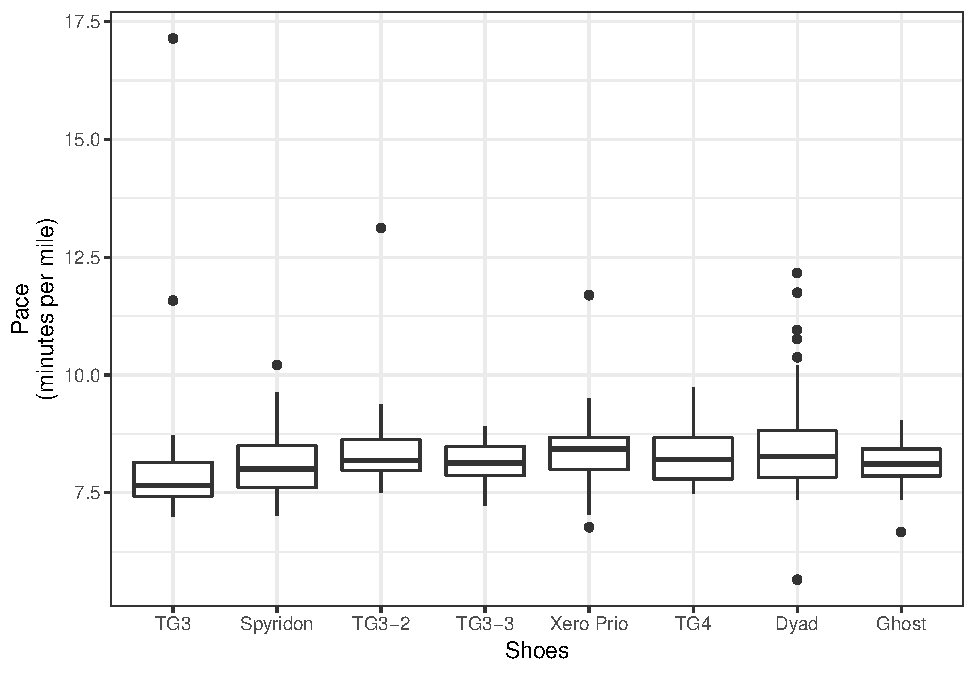
\includegraphics{my_running_data_files/figure-latex/unnamed-chunk-6-1.pdf}

There might be a difference here. To see if there is a
statistically-significant difference, I'll run a basic analysis of
variance (ANOVA).

\begin{Shaded}
\begin{Highlighting}[]
\NormalTok{anova_shoes <-}\StringTok{ }\KeywordTok{aov}\NormalTok{(Pace }\OperatorTok{~}\StringTok{ }\NormalTok{Activity.Gear, }\DataTypeTok{data =}\NormalTok{ shoes_df)}
\KeywordTok{summary}\NormalTok{(anova_shoes)}
\end{Highlighting}
\end{Shaded}

\begin{verbatim}
##                Df Sum Sq Mean Sq F value Pr(>F)  
## Activity.Gear   7  14.71  2.1011   2.367 0.0226 *
## Residuals     334 296.45  0.8876                 
## ---
## Signif. codes:  0 '***' 0.001 '**' 0.01 '*' 0.05 '.' 0.1 ' ' 1
\end{verbatim}

This shows that there is some significant difference in at least two
different pairs of shoes, however, this does not tell use which shoes
have significantly different average paces. In order to find that
information, we will need to use something like Tukey's Honestly
Significant Difference Test.

\begin{Shaded}
\begin{Highlighting}[]
\NormalTok{tukey_test <-}\StringTok{ }\KeywordTok{TukeyHSD}\NormalTok{(anova_shoes)}
\NormalTok{tukey_test}
\end{Highlighting}
\end{Shaded}

\begin{verbatim}
##   Tukey multiple comparisons of means
##     95% family-wise confidence level
## 
## Fit: aov(formula = Pace ~ Activity.Gear, data = shoes_df)
## 
## $Activity.Gear
##                             diff         lwr         upr     p adj
## Ghost-Dyad         -0.4011169249 -1.28368211  0.48144826 0.8631030
## Spyridon-Dyad      -0.3595597242 -0.91459663  0.19547718 0.4997251
## TG3-Dyad           -0.5366822583 -0.99732359 -0.07604092 0.0101903
## TG3-2-Dyad         -0.1196867894 -0.65575490  0.41638133 0.9974443
## TG3-3-Dyad         -0.3601830504 -0.93779258  0.21742648 0.5504586
## TG4-Dyad           -0.1499766619 -0.85966112  0.55970779 0.9981989
## Xero Prio-Dyad     -0.0423088266 -0.60261180  0.51799414 0.9999983
## Spyridon-Ghost      0.0415572006 -0.91001573  0.99313013 1.0000000
## TG3-Ghost          -0.1355653334 -1.03535171  0.76422104 0.9998043
## TG3-2-Ghost         0.2814301355 -0.65920481  1.22206508 0.9847405
## TG3-3-Ghost         0.0409338745 -0.92397951  1.00584726 1.0000000
## TG4-Ghost           0.2511402630 -0.79818195  1.30046247 0.9960444
## Xero Prio-Ghost     0.3588080983 -0.59584602  1.31346222 0.9459103
## TG3-Spyridon       -0.1771225340 -0.75915361  0.40490854 0.9831562
## TG3-2-Spyridon      0.2398729349 -0.40350779  0.88325366 0.9481472
## TG3-3-Spyridon     -0.0006233261 -0.67900560  0.67775894 1.0000000
## TG4-Spyridon        0.2095830624 -0.58428202  1.00344814 0.9927616
## Xero Prio-Spyridon  0.3172508977 -0.34645774  0.98095953 0.8290033
## TG3-2-TG3           0.4169954689 -0.14697549  0.98096642 0.3217738
## TG3-3-TG3           0.1764992079 -0.42709584  0.78009426 0.9866574
## TG4-TG3             0.3867055964 -0.34428431  1.11769550 0.7418769
## Xero Prio-TG3       0.4943734317 -0.09268162  1.08142848 0.1712335
## TG3-3-TG3-2        -0.2404962610 -0.90344842  0.42245590 0.9551390
## TG4-TG3-2          -0.0302898725 -0.81101058  0.75043084 1.0000000
## Xero Prio-TG3-2     0.0773779628 -0.57055121  0.72530714 0.9999593
## TG4-TG3-3           0.2102063885 -0.59960135  1.02001412 0.9934705
## Xero Prio-TG3-3     0.3178742238 -0.36482334  1.00057178 0.8474831
## Xero Prio-TG4       0.1076678353 -0.68988794  0.90522361 0.9999065
\end{verbatim}

This shows that only two shoes have average paces that are significantly
different: the TG3 (Merrill Trail Glove 3), and the Brooks Dyad. This is
likely because I purchased the Dyad in order to recover from my planar
fasciitis in late 2018.

\hypertarget{conclusion}{%
\subsection{Conclusion}\label{conclusion}}

I found that, while my pace was getting slower through the beginning of
2019, this is probably because my runs were getting longer and/or I was
recovering from an injury. Otherwise, there does not seem to be a
significant linear trend through time in terms of my average pace. From
this, the take-home lesson seems to be, ``Try to avoid an injury.''


\end{document}
